\section{Punto de Vista de Capas}

El punto de vista por capas muestra las diferentes capas y aspectos de la arquitectura empresarial en un modelo. Existen dos categorías de capas, capas dedicadas y capas de servicio. Las capas son resultado de la relación de “agrupación” para un particionado natural de todo el conjunto de objetos y relaciones que pertenecen al modelo. La infraestructura, la aplicación, los procesos y los actores/roles pertenecen a la primera categoría. El principio estructural es que cada capa dedicada expone por medio de una relación de “realización” una capa de servicios, las cuales serán “usadas por” la siguiente capa dedicadas. A partir de esto se puede separar la estructura interna y la organización de cada capa dedicada de su comportamiento externo observable expresado como el servicio que esa capa dedicada realiza. 

\subsection{Modelo de Capas}
\begin{figure}[h!]
	\centering
	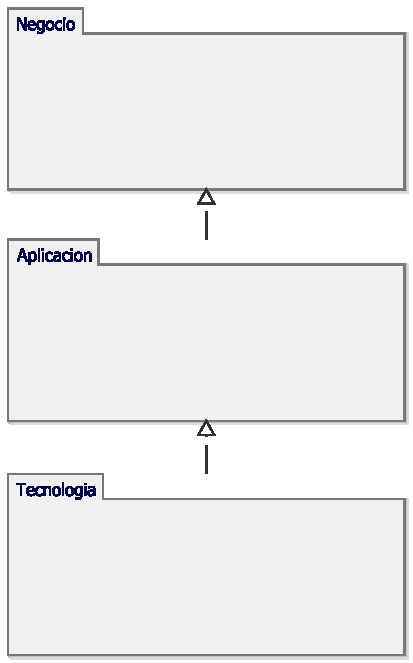
\includegraphics[width=.5\linewidth]{imgs/modelo/Capas}
	\caption{Modelo de Capas}
\end{figure}

El modelo de capas muestra como los servicios de negocio, aplicación e infraestructura son integrados por medio de sus modelos intermedios: Se muestran los servicios de negocio principales y los procesos de negocio que los realizan, estos procesos están asociados con servicios de aplicación específicos que a su vez son realizados por componentes de aplicación definidos para la arquitectura del sistema de software. Los componentes se encuentran soportados en servicios de infraestructura realizados por nodos de infraestructura y aplicaciones de software concretas.


\subsection{Caso punto de vista de Capas}
\begin{figure}[h!]
	\centering
	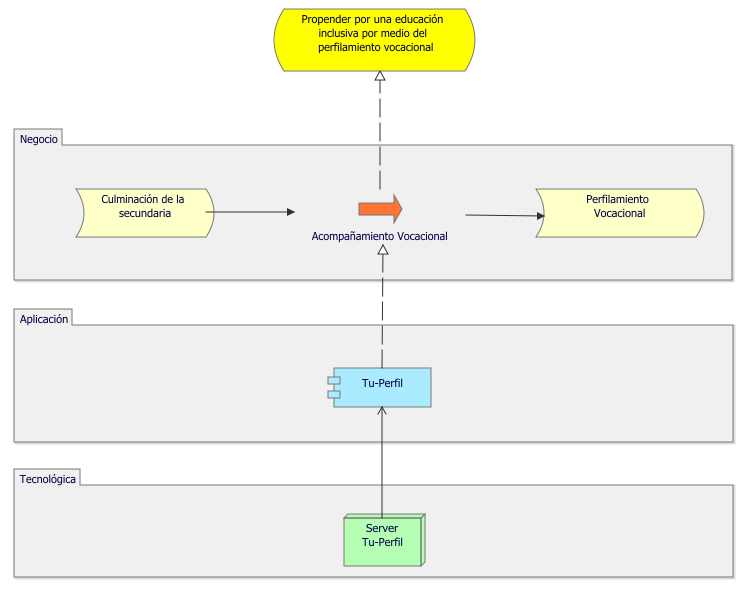
\includegraphics[width=1\linewidth]{imgs/caso/CapasTuPerfil}
	\caption{Caso de Capas}
\end{figure}

Para el caso del proyecto Tu-Perfil, el punto de vista de capas inicia con el objetivo central del proyecto Tu-Perfil, el cual es propender por una educación inclusiva por medio del perfilamiento vocacional y se conecta con tres capas fundamentales en el proceso de construcción del proyecto, estas capas son: la capa de negocio en la cual se especifica lo más relevante trabajado en esos puntos de vista pertenencientes a la capa de negocio contando con el proceso principal del acompañamiento vocacional precedido por la culminación de la secundaria y lo sucede el perfilamiento vocacional. Sigue la capa de aplicación con el paquete principal de Tu-Perfil y la capa tecnológica con el servidor Tu-Perfil.

\clearpage